%% ---------------------------------------------------------------------------
%% Flagship INTRODUCTION figure (Figure 1) -- v4
%% "Concepts Whisper: Spectral Anti-Concentration and the Dual Geometry
%%  of Transformer Representations" (EMNLP main, camera-ready)
%%
%% Standalone TikZ/PGF -- compile with:  tectonic dual_geometry_v4.tex
%% Produces a tightly-cropped vector PDF; the paper does
%%   \includegraphics[width=\textwidth]{figures/intro/dual_geometry_v4.pdf}
%% and does NOT depend on this file's preamble.
%% ---------------------------------------------------------------------------
\documentclass[tikz,border=2pt]{standalone}

\usepackage[T1]{fontenc}
\usepackage{helvet}
\renewcommand{\familydefault}{\sfdefault}
\usepackage{sansmathfonts}   % sans-serif math to match the modern sans look

\usetikzlibrary{arrows.meta,positioning,calc,backgrounds,shadings,fadings}

% -- Okabe-Ito colorblind-safe palette (groups also differ by SHAPE + POSITION)
\definecolor{head}{HTML}{D55E00}   % vermilion  : vocabulary / high-variance head
\definecolor{headf}{HTML}{F7DAC6}  % light warm fill
\definecolor{tail}{HTML}{0072B2}   % steel blue : activation / low-variance tail
\definecolor{tailf}{HTML}{CFE4F1}  % light cool fill
\definecolor{spec}{HTML}{9AA0A6}   % neutral grey eigen-spectrum
\definecolor{ink}{HTML}{1A1A1A}    % near-black text / arrow
\definecolor{mute}{HTML}{5F6368}   % muted secondary text
\definecolor{faint}{HTML}{8A9096}  % faint axis / annotation grey
\definecolor{grid}{HTML}{D2D6DA}   % faint borders

% ---------------------------------------------------------------------------
% Precomputed, reproducible marker positions (Python/NumPy seed=7).
% HEAD = vocabulary contrasts -> tight cluster (CONCENTRATE), squares.
\def\headpts{2.751/2.150,2.905/2.832,2.607/2.416,2.487/3.086,2.514/3.028,%
2.334/2.857,2.781/2.250,3.147/2.681,2.494/2.926,2.427/3.007,2.905/2.285,%
2.836/2.711,2.805/2.561,2.366/2.546,2.735/3.280,3.012/2.546,2.151/2.934,%
2.512/3.192,1.961/2.658,2.179/2.894}
% TAIL = activation directions -> spread out (ANTI-CONCENTRATE), three methods.
\def\tailO{14.306/2.887,12.157/2.764,14.113/2.435,12.910/3.701,13.502/2.871,%
9.731/4.010,12.339/3.271,12.145/3.300,14.254/3.362,11.295/3.435,12.669/2.436,%
9.544/2.987}                                          % diff-of-means (circle)
\def\tailD{10.589/2.400,11.534/3.756,10.350/3.980,14.813/3.867,10.447/3.232,%
13.096/2.426,10.942/2.516,14.270/3.913,13.041/3.199} % SAE feature (diamond)
\def\tailT{10.247/3.039,14.328/3.191,12.921/2.762,12.504/3.578,11.382/2.198,%
11.584/2.857,10.589/2.208,9.421/2.383,14.282/3.988}  % linear probe (triangle)

% Marker drawing styles (soft rounded, white halo so clusters read cleanly).
\tikzset{
  sq/.style   ={draw=white,line width=0.6pt,fill=head,rounded corners=0.7pt},
  circ/.style ={draw=white,line width=0.6pt,fill=tail},
  dia/.style  ={draw=white,line width=0.6pt,fill=tail,line join=round},
  tri/.style  ={draw=white,line width=0.6pt,fill=tail,line join=round},
}

\begin{document}
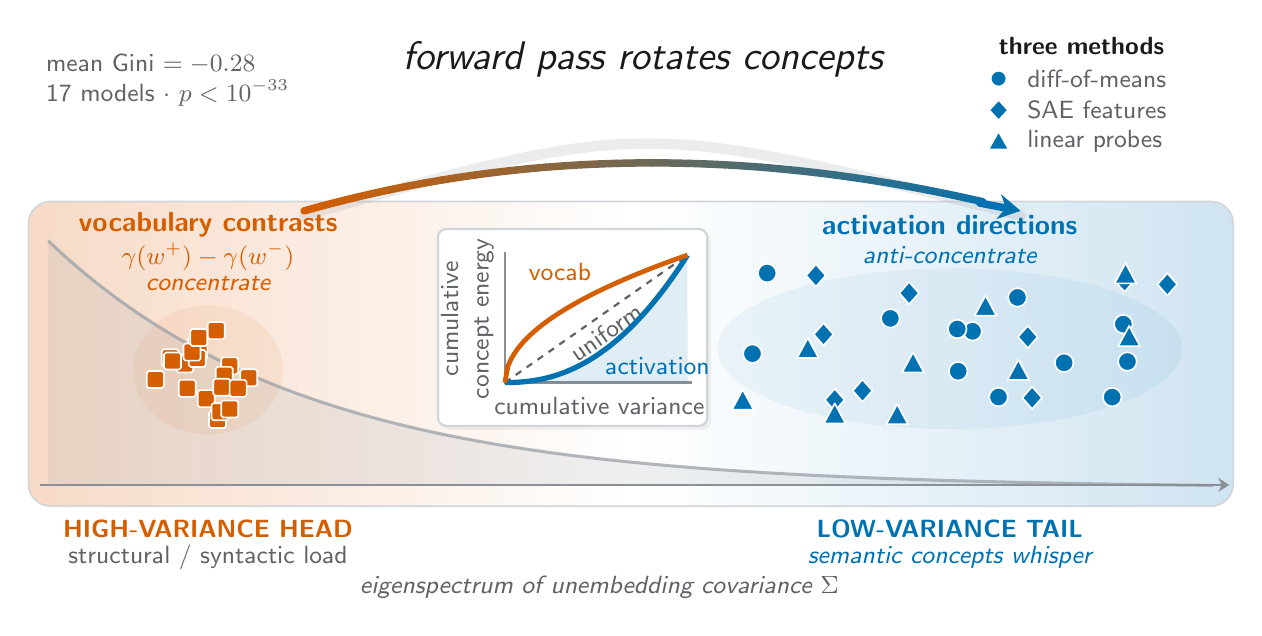
\begin{tikzpicture}[x=1cm,y=1cm]

  %% ==== background region band: warm head -> quiet centre -> cool tail ======
  \begin{scope}
    \clip[rounded corners=8pt] (0.35,1.05) rectangle (15.65,4.92);
    \shade[left color=headf,right color=tailf,middle color=white]
      (0.35,1.05) rectangle (15.65,4.92);
  \end{scope}
  \draw[grid,line width=0.6pt,rounded corners=8pt]
      (0.35,1.05) rectangle (15.65,4.92);

  %% ==== subtle spread cues: tight head hull vs. diffuse tail hull ===========
  \fill[head,opacity=0.07] (2.63,2.78) ellipse (0.95cm and 0.82cm);
  \fill[tail,opacity=0.055] (12.05,3.05) ellipse (2.95cm and 1.02cm);

  %% ==== grey eigen-spectrum "scree": loud head -> quiet tail ===============
  \path[fill=spec,fill opacity=0.16]
    plot[domain=0:1,samples=160]
      ({0.6+14.8*\x},{1.32+3.10*((exp(-4.4*\x)*(1-0.10*\x)+0.012-0.025)/0.987)})
    -- (15.4,1.32) -- (0.6,1.32) -- cycle;
  \draw[spec,line width=1.1pt,opacity=0.75]
    plot[domain=0:1,samples=160]
      ({0.6+14.8*\x},{1.32+3.10*((exp(-4.4*\x)*(1-0.10*\x)+0.012-0.025)/0.987)});

  %% ==== spectrum axis (high-variance -> low-variance) ======================
  \draw[faint,line width=1.0pt,-{Stealth[length=4pt,width=5pt]}]
      (0.5,1.32) -- (15.6,1.32);

  %% ==== marker clusters ====================================================
  % HEAD: vocabulary contrasts (vermilion squares), concentrated
  \foreach \px/\py in \headpts {
    \fill[sq] (\px-0.108,\py-0.108) rectangle (\px+0.108,\py+0.108);
  }
  % TAIL: activation directions, three independent methods, spread out
  \foreach \px/\py in \tailO { \fill[circ] (\px,\py) circle (0.118); }
  \foreach \px/\py in \tailD {
    \fill[dia] (\px,\py+0.142)--(\px+0.125,\py)--(\px,\py-0.142)--(\px-0.125,\py)--cycle; }
  \foreach \px/\py in \tailT {
    \fill[tri] (\px,\py+0.148)--(\px+0.138,\py-0.108)--(\px-0.138,\py-0.108)--cycle; }

  %% ==== the forward-pass rotation arrow (the protagonist) ==================
  %% A single sweeping arc whose stroke grades vermilion -> steel blue, so the
  %% arrow itself *encodes* the head->tail rotation of concept geometry.
  \def\Ax{3.85}\def\Ay{4.80}   % start (above head cluster)
  \def\Bx{8.15}\def\By{6.02}   % control (peak)
  \def\Cx{12.95}\def\Cy{4.80}  % end   (above tail cluster)
  % soft drop shadow for depth
  \draw[spec,line width=3.8pt,opacity=0.20,line cap=round]
      (\Ax,\Ay-0.06) .. controls (\Bx,\By-0.06) .. (\Cx,\Cy-0.06);
  % graded stroke (quadratic Bezier sampled in short colored segments)
  \foreach \i in {0,...,37}{
    \pgfmathsetmacro{\ta}{\i/40}
    \pgfmathsetmacro{\tb}{(\i+1)/40}
    \pgfmathsetmacro{\xa}{(1-\ta)*(1-\ta)*\Ax + 2*(1-\ta)*\ta*\Bx + \ta*\ta*\Cx}
    \pgfmathsetmacro{\ya}{(1-\ta)*(1-\ta)*\Ay + 2*(1-\ta)*\ta*\By + \ta*\ta*\Cy}
    \pgfmathsetmacro{\xb}{(1-\tb)*(1-\tb)*\Ax + 2*(1-\tb)*\tb*\Bx + \tb*\tb*\Cx}
    \pgfmathsetmacro{\yb}{(1-\tb)*(1-\tb)*\Ay + 2*(1-\tb)*\tb*\By + \tb*\tb*\Cy}
    \pgfmathtruncatemacro{\mix}{100-100*\ta}
    \draw[line width=2.7pt,line cap=round,color=head!\mix!tail] (\xa,\ya)--(\xb,\yb);
  }
  % steel-blue arrowhead (final short segment along the tangent)
  \draw[line width=2.7pt,line cap=round,color=tail,-{Stealth[length=8pt,width=9pt]}]
      (12.43,4.90) -- (\Cx,\Cy);

  %% ==== headline title above the arc =======================================
  \node[ink,font=\itshape\Large] at (8.15,6.72)
      {forward pass rotates concepts};

  %% ==== cluster captions + the core finding verbs ==========================
  % head (vermilion vocabulary contrasts -- a real finding)
  \node[head,font=\bfseries\normalsize,align=center] at (2.63,4.62)
      {vocabulary contrasts};
  \node[head,font=\small] at (2.63,4.22) {$\gamma(w^{+})-\gamma(w^{-})$};
  \node[head,font=\itshape\small] at (2.63,3.88) {concentrate};
  % tail (steel-blue activation directions -- the protagonist)
  \node[tail,font=\bfseries\normalsize] at (12.05,4.62)
      {activation directions};
  \node[tail,font=\itshape\small] at (12.05,4.24) {anti-concentrate};

  %% ==== inset: empirical cumulative-energy signature (self-contained) ======
  \begin{scope}
    % card + soft shadow
    \fill[black,opacity=0.05,rounded corners=3pt] (5.60,2.02) rectangle (9.02,4.52);
    \filldraw[fill=white,draw=grid,line width=0.8pt,rounded corners=3pt]
        (5.55,2.07) rectangle (8.97,4.57);
    % plot geometry: x0=6.40,x1=8.72 ; y0=2.62,y1=4.24
    % L-shaped axes
    \draw[faint,line width=0.8pt] (6.40,4.28) -- (6.40,2.62) -- (8.78,2.62);
    % uniform reference diagonal
    \draw[mute,line width=0.8pt,dash pattern=on 2.4pt off 2.4pt]
        (6.40,2.62) -- (8.72,4.24);
    \node[mute,font=\small,rotate=34.8,anchor=north] at (7.55,3.45) {uniform};
    % activation curve bows BELOW the diagonal -> anti-concentration
    \path[fill=tail,fill opacity=0.12]
      plot[domain=0:1,samples=60,variable=\t] ({6.40+2.32*\t},{2.62+1.62*pow(\t,2.25)})
      -- (8.72,2.62) -- (6.40,2.62) -- cycle;
    \draw[tail,line width=1.9pt]
      plot[domain=0:1,samples=60,variable=\t] ({6.40+2.32*\t},{2.62+1.62*pow(\t,2.25)});
    % vocabulary curve bows ABOVE the diagonal -> concentration
    \draw[head,line width=1.7pt]
      plot[domain=0:1,samples=60,variable=\t] ({6.40+2.32*\t},{2.62+1.62*sqrt(\t)});
    % inline curve labels
    \node[head,font=\small,anchor=west] at (6.58,4.02) {vocab};
    \node[tail,font=\small,anchor=west] at (7.55,2.83) {activation};
    % axis labels -- padded, no overlap with axes or curves
    \node[mute,font=\small,align=center,rotate=90] at (5.92,3.43)
        {cumulative\\concept energy};
    \node[mute,font=\small] at (7.60,2.32) {cumulative variance};
  \end{scope}

  %% ==== legend: three independent methods (top-right) ======================
  \begin{scope}[shift={(12.55,6.48)}]
    \node[ink,font=\small\bfseries,anchor=west] at (0.0,0.42) {three methods};
    \fill[circ] (0.12,0.0) circle (0.10);
    \node[mute,font=\small,anchor=west] at (0.36,0.0) {diff-of-means};
    \fill[dia] (0.12,-0.40+0.13)--(0.24,-0.40)--(0.12,-0.40-0.13)--(0.0,-0.40)--cycle;
    \node[mute,font=\small,anchor=west] at (0.36,-0.40) {SAE features};
    \fill[tri] (0.12,-0.80+0.13)--(0.25,-0.80-0.10)--(-0.01,-0.80-0.10)--cycle;
    \node[mute,font=\small,anchor=west] at (0.36,-0.80) {linear probes};
  \end{scope}

  %% ==== headline statistic (subtle, top-left) ==============================
  \node[mute,font=\small,align=left,anchor=north west] at (0.45,6.92)
      {mean Gini $=-0.28$\\17 models\,\,$\cdot$\,\,$p<10^{-33}$};

  %% ==== region labels + framing (below the axis) ===========================
  % head: named finding; the functional structural reading is SECONDARY/muted
  \node[head,font=\small\bfseries] at (2.63,0.76) {HIGH-VARIANCE HEAD};
  \node[mute,font=\small] at (2.63,0.40) {structural / syntactic load};
  % tail: the robust protagonist -- the paper's title nod is supported
  \node[tail,font=\small\bfseries] at (12.05,0.76) {LOW-VARIANCE TAIL};
  \node[tail,font=\small\itshape] at (12.05,0.40) {semantic concepts whisper};

  %% ==== axis caption =======================================================
  \node[mute,font=\small\itshape] at (7.6,0.02)
      {eigenspectrum of unembedding covariance $\Sigma$};

\end{tikzpicture}
\end{document}
